\documentclass{article}
%\usepackage{graphics}
\usepackage{thmtools}
\usepackage{amssymb}
\usepackage{amsmath}
\usepackage{graphicx}
\declaretheorem{theorem}
\def\qed{\hfill$\square$}

\begin{document}

\title{Složitost operace Make heap}
\date{}
\maketitle

\section{Kontext}

Halda je užitečná datová struktura. Avšak mnozí tvrdí, že ji lze z neseřazeného pole nainicializovat v čase $O(n)$.
To nemusí na první pohled dávat smysl --- kdyby totiž člověk vytvářel haldu postupným přidáváním prvků, tak by její vytvoření mělo složitost $O(n \log(n))$.
Tak jak to tedy je?

Tvoření haldy neprobíhá postupným přidáváním prvků, ale opravy h-vlastnosti zespodu.
Když si představíme haldu jako strom (viz obrázek), tak se od spodu bere každý podstrom a udělá se z něj halda.
Protože se prvky berou odspodu, tak vždy víme, že synové podstromu, ze kterého se snažíme udělat haldu už haldy jsou (žlutý a zelený), a tak stačí pouze prvku na vrcholku upravit h-vlastnost (modrý).

\begin{figure}
    \centering
    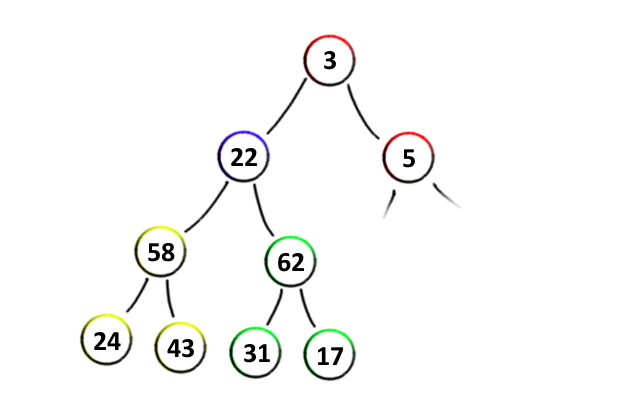
\includegraphics[width=0.5\textwidth]{make_heap.png}
    \caption{Podstromy haldy při provádění make heap operace}%
\end{figure}

\begin{theorem}
Vytvoření haldy má složitost $O(n)$.
\end{theorem}

\section{Důkaz}
Pro všech n prvků musíme opravit h-vlastnost --- to znamená prohodit jej s větším z potomků, pokud je prvek menší než alespoň jeden z jeho potomků.
Tato operace se potom volá rekurzivně a víme, že se provede maximálně g krát, kde g je výška uzlu.
Doplňme haldu tak, aby všechny listy ležely ve stejné hloubce.
Tímto nezvětšíme velikost haldy o více jak n/2.
Nyní spočteme kolik uzlů je v jedné výšce g.
Protože je halda úplný binární strom, tak se s hloubkou počet uzlů dvojnásobí.
Výška je však pojem opačný, takže začneme s vysokým počtem uzlů, který se bude se zvyšující se výškou dělit dvěma.
Tedy: ve výšce g a hloubkce stromu h je \[
    \frac{2^h}{2^g}.
\]

Z toho co jsme si doposud řekli vyplývá, že počet operací pro celé jedno patro je \[
    g \frac{2^h}{2^g}.
\]

Pro sečtení všech pater použijeme sumu \[
    \sum_{g=1}^h g \frac{2^h}{2^g}.
\]

Hodnota h není v sumě proměnnou a tak ji můžeme vytknout.
\[
    2^h \sum_{g=1}^h \frac{g}{2^g}
\]

Nyní se zaměříme pouze na člen sumy.
Víme, že všechny členy sumy jsou nezáporné, a tak je suma určitě menší než součet s intervalem do nekonečna.
Tuto sumu můžeme upravit vytknutím 1/2.
Dále jen změníme index sumy.
Potom sumu rozložíme na dvě, podle čitatele podílu.
Nakonec z první sumy odebereme prvek pro $g=0$, protože výraz vychází 0, ten sumu nijak nemění.

\begin{align*}
    \sum_{g=1}^h \frac{g}{2^g} \leq &\sum_{g=1}^\infty \frac{g}{2^g} = \frac{1}{2} \sum_{g=1}^\infty \frac{g}{2^{g-1}} \\
    = &\frac{1}{2} \sum_{g=0}^\infty \frac{g + 1}{2^g} = \frac{1}{2} \left(\sum_{g=0}^\infty \frac{g}{2^g} + \sum_{g=0}^\infty \frac{1}{2^g}\right) \\
    = &\frac{1}{2} \left(\sum_{g=1}^\infty \frac{g}{2^g} + \sum_{g=0}^\infty \frac{1}{2^g}\right)
\end{align*}

Z rovnice dostáváme vztah
\[
    \sum_{g=1}^\infty \frac{g}{2^g} = \frac{1}{2} \left(\sum_{g=1}^\infty \frac{g}{2^g} + \sum_{g=0}^\infty \left(\frac{1}{2}^g\right)\right)
\]

Po substituci SUM výraz zjednodušíme.
\[
    a = \frac{1}{2} \cdot (a + b) \rightarrow a = a/2 + b/2 \rightarrow a = b
\]

Zpátky dostáváme následující vztah.
\[
    \sum_{g=1}^\infty \frac{g}{2^g} = \sum_{g=0}^\infty \frac{1}{2^g}
\]

Pravá strana výrazu má tvar geometrické řady, pro kterou je známý součtový vzorec.
Mnoho lidí umí tuto řadu sečíst i bez součtového vzorce.
\[
    \sum_{g=0}^\infty \frac{1}{2^g} = 1 + \frac{1}{2} + \frac{1}{4} + \frac{1}{8} + \cdots = 2
\]

Z toho vyplývá, že \[
    \sum_{g=1}^h \frac{g}{2^g} < 2.
\]

A tak součet všech operací přes všechny prvky všech pater haldy je
\[
    2^h \sum_{g=1}^h \frac{g}{2^g} < 2^{h+1}.
\]

A protože pro hloubku úplného binárního stromu platí $h = \log(n)$, dostáváme složitost make heap
\[
    O(2^h) = O(2^{\log(n)}) = O(n).
\]

Což jsme chtěli dokázat. \qed\


%## Zdroje

%* [Základ důkazu](https://en.wikipedia.org/w/index.php?title=Binary_heap&oldid=688333923#Building_a_heap)
%* [Vysvětlení součtu](http://austinrochford.com/posts/2014-01-30-math-heap-linear-time.html)

\end{document}  %End of document.
